\section{The physics behind X-ray diffraction}

Max von Laue discovered the phenomena of diffraction of X-rays by crystals, for which he was awarded the Nobel Prize in Physics in 1914. Laue viewed the three-dimensional periodic arrangement of atoms in a crystal as a 3D diffraction grating, and thereby derived a condition which needs to be satisfied for the diffraction of X-rays to take place.

Sir William Henry Bragg and William Lawrence Bragg furthered the physics of X-ray diffraction. Lawrence Bragg, in contrast to Laue's work, viewed the layers (planes) of atoms in the crystal lattice as reflecting surfaces, and X-ray beams reflecting off consecutive planes would interfere constructively if a certain condition was satisfied. This theory is not true in the physical sense -- planes of atoms do not reflect X-rays as such -- but it is correct in the geometrical sense, and we can arrive at Bragg's Law if we start from Laue's condition. The Braggs were jointly awarded the Nobel prize in Physics in 1915 for their work in X-ray crystallography.

\subsection{Bragg's Analysis}
	
	\begin{figure}
	\centering
	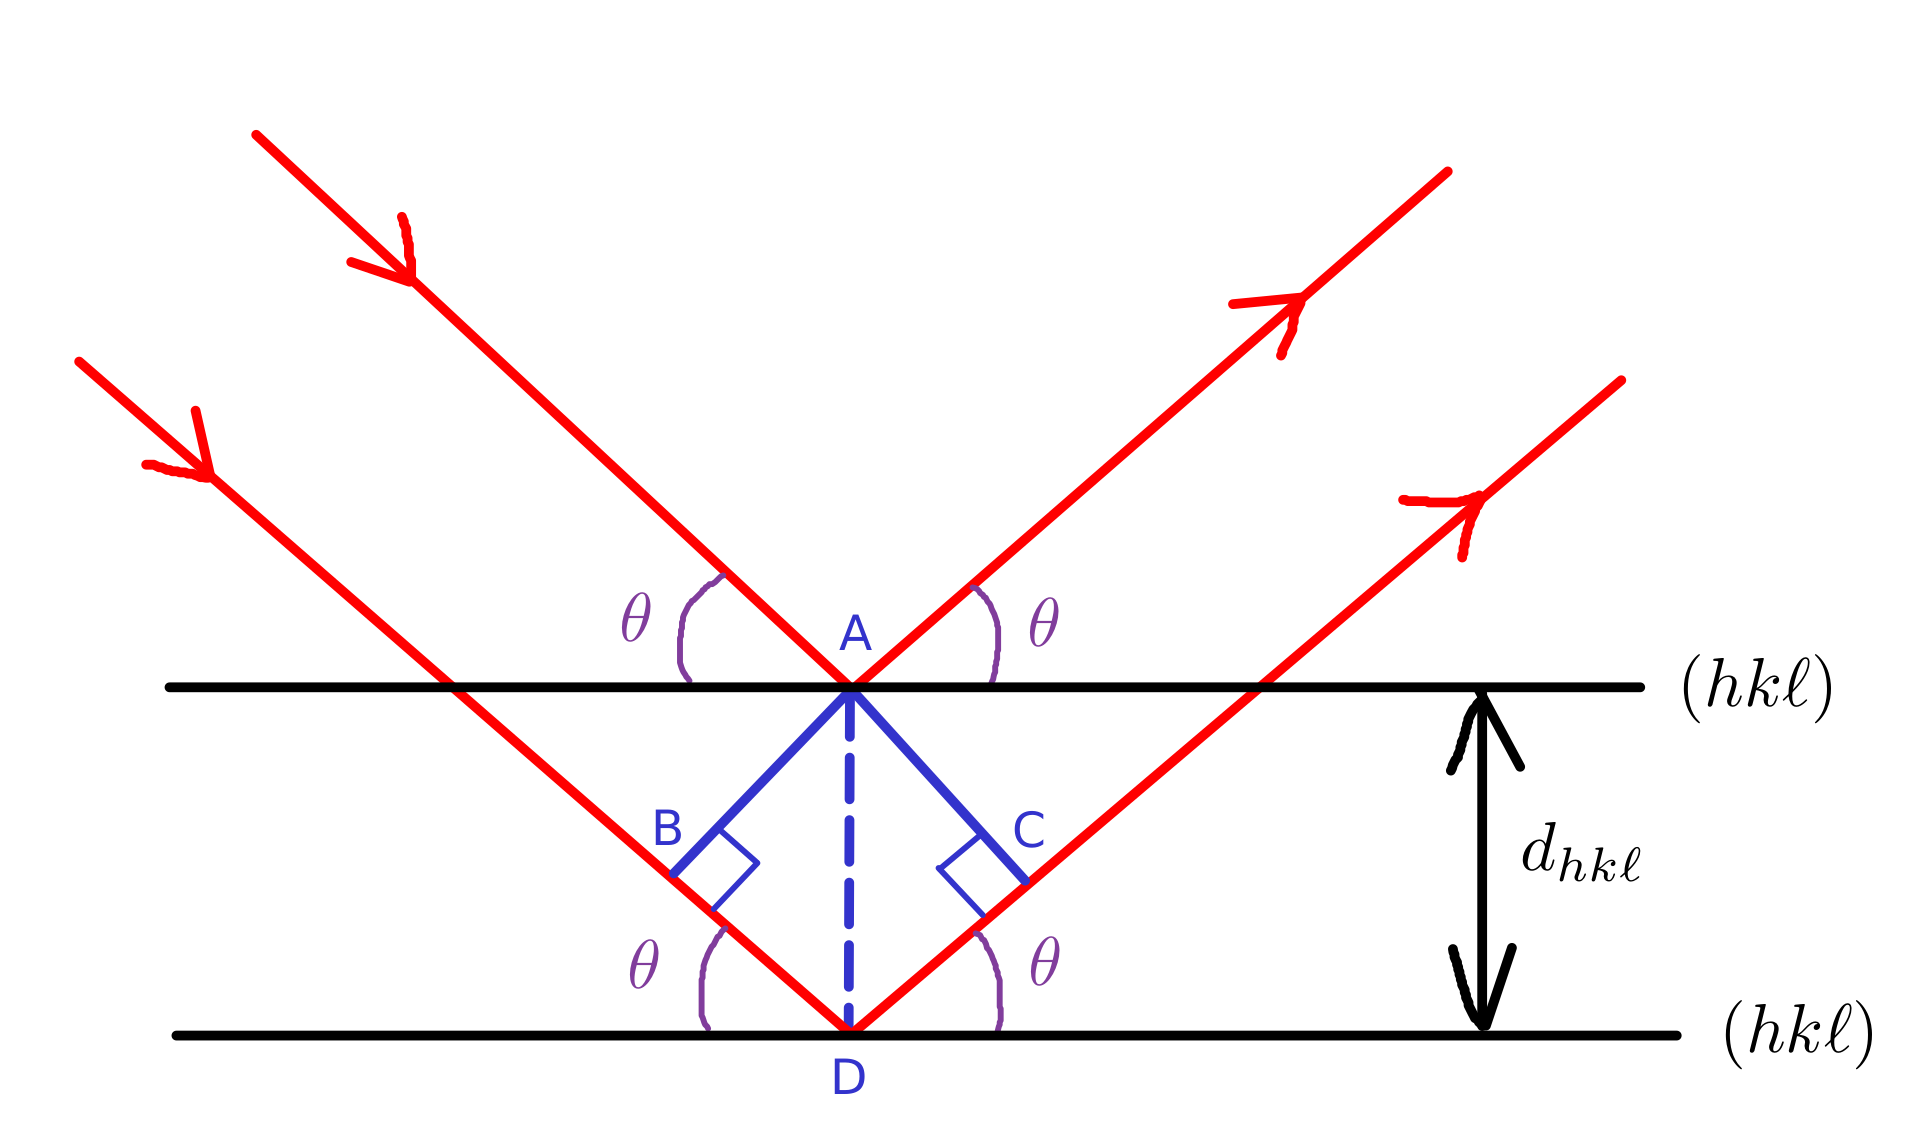
\includegraphics[scale=0.15]{bragg_law.png}
	\caption{\label{fig:bragg_law}X-ray beam is incident on a set of planes with Miller indices $(hk\ell),$ as shown. We draw perpendiculars $\mathrm{AB}$ and $\mathrm{AC}$. $d_{hk\ell}$ is the perpendicular distance between two planes with the same Miller indices $(hk\ell).$}
	\end{figure}

	Derivation of Bragg's Law is straightforward. Referring to figure~\ref{fig:bragg_law}, the path difference,%
%	
	\begin{align}
	\mathrm{P.D.} &= \mathrm{BD} + \mathrm{DC} \nonumber\\
				&= 2 d_{hk\ell} \sin \theta.
	\end{align}
	
	For constructive interference,%
%	
	\begin{align}
	&\phantom{\implies} \mathrm{P.D.} = n \lambda,\quad n \in \mathbb{Z} \nonumber\\
	&\implies \boxed{2 d_{hk\ell} \sin \theta = n \lambda}
	\end{align}
%	
	which is Bragg's Law for X-ray diffraction. $n$ is the order of diffraction or reflection.
	
%***************************************************************************************************
	
\subsection{Laue's analysis}

	\begin{figure}
	\centering
	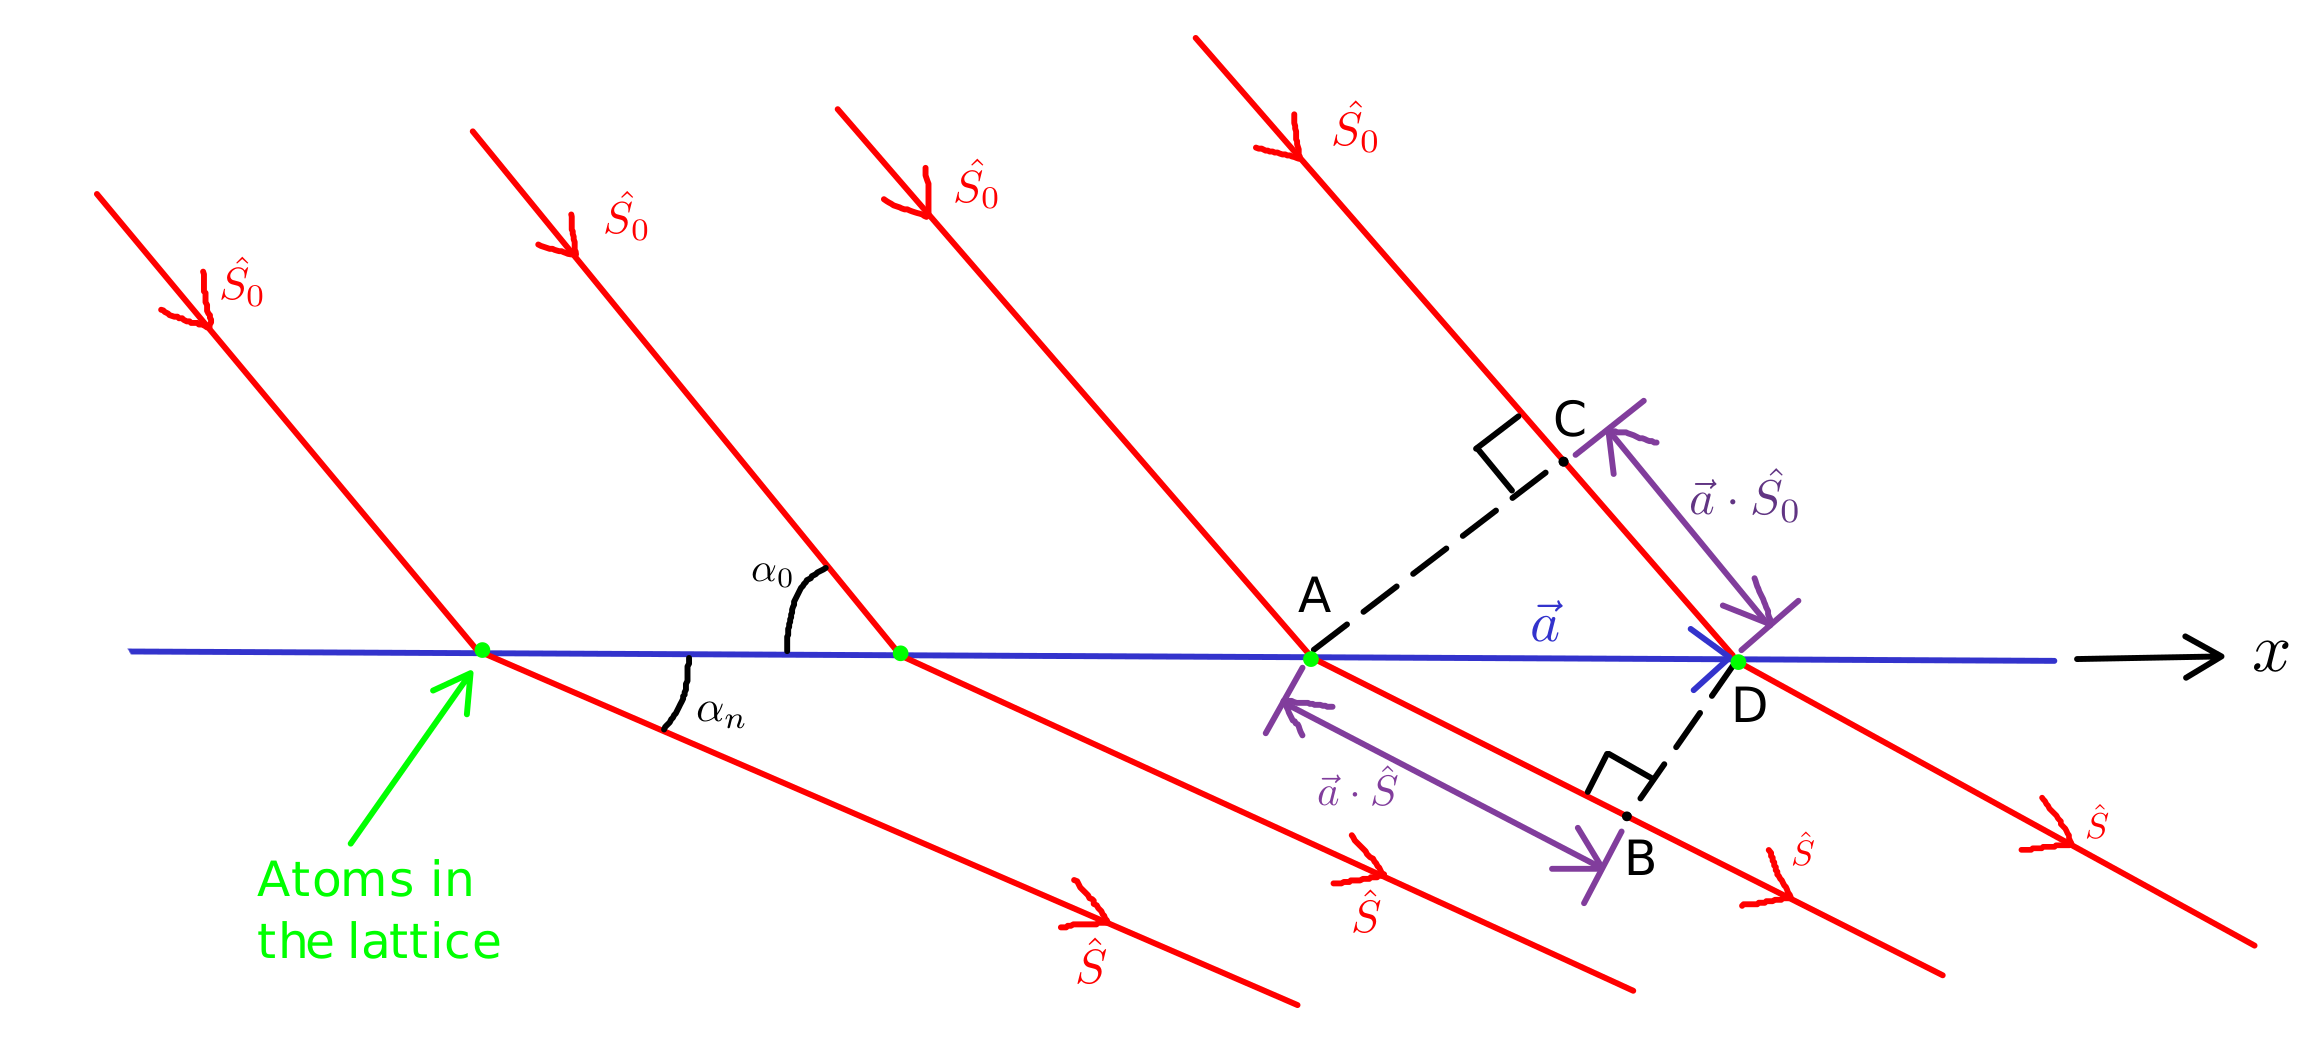
\includegraphics[scale=0.17]{laue_analysis.png}
	\caption{\label{fig:laue_analysis}Diffraction from a lattice row along the $x$ axis. The incident and diffracted beams make angles $\alpha_0$ and $\alpha_n$ respectively with the lattice row. $\vec{a}$ is the lattice translation vector.}
	\end{figure}
	
	Consider a simple crystal with one atom as the basis, as shown in figure~\ref{fig:laue_analysis}. The atoms are regarded as the scattering centres from which the diffraction takes place. $\hat{S_0}$ and $\hat{S}$ are two unit vectors in the direction of the incident and diffracted beam, respectively. The lattice spacing is $a$.
	
	The path difference,%
%		
		\begin{align}
		\mathrm{P.D.} &= \mathrm{AB - CD}, \nonumber\\
					  &= a \qty( \cos \alpha_n - \cos \alpha_0 ) \\
					  &= \va{a} \cdot \qty( \vu{S} - \vu{S_0} ),
		\end{align}%
%		
	has to be an integer multiple of wavelength for constructive interference.%
%		
		\begin{equation}
		\therefore \boxed{a \qty( \cos \alpha_n - \cos \alpha_0 ) = \va{a} \cdot \qty( \vu{S} - \vu{S_0} ) = n_x \lambda,} \quad n_x \in \mathbb{Z}. \label{eq:1st_laue_eqn}
		\end{equation}
		
	Eqn.~\eqref{eq:1st_laue_eqn} is the \textbf{first Laue equation}.
	
	This path difference is still valid if the diffracted beam, instead of being below the row of atoms, is above it, or is out of the plane of the paper itself. Therefore, all diffracted beams with the same path difference occur at the same angle to the atom row. Thus, all diffracted beams lie on the surface of a cone, known as the \bfnt{Laue cone}, centred on the atom row with semi-apex angle $\alpha_n.$ This is illustrated in figure~\ref{fig:laue_cones}.
	
	\begin{figure}
	\centering
	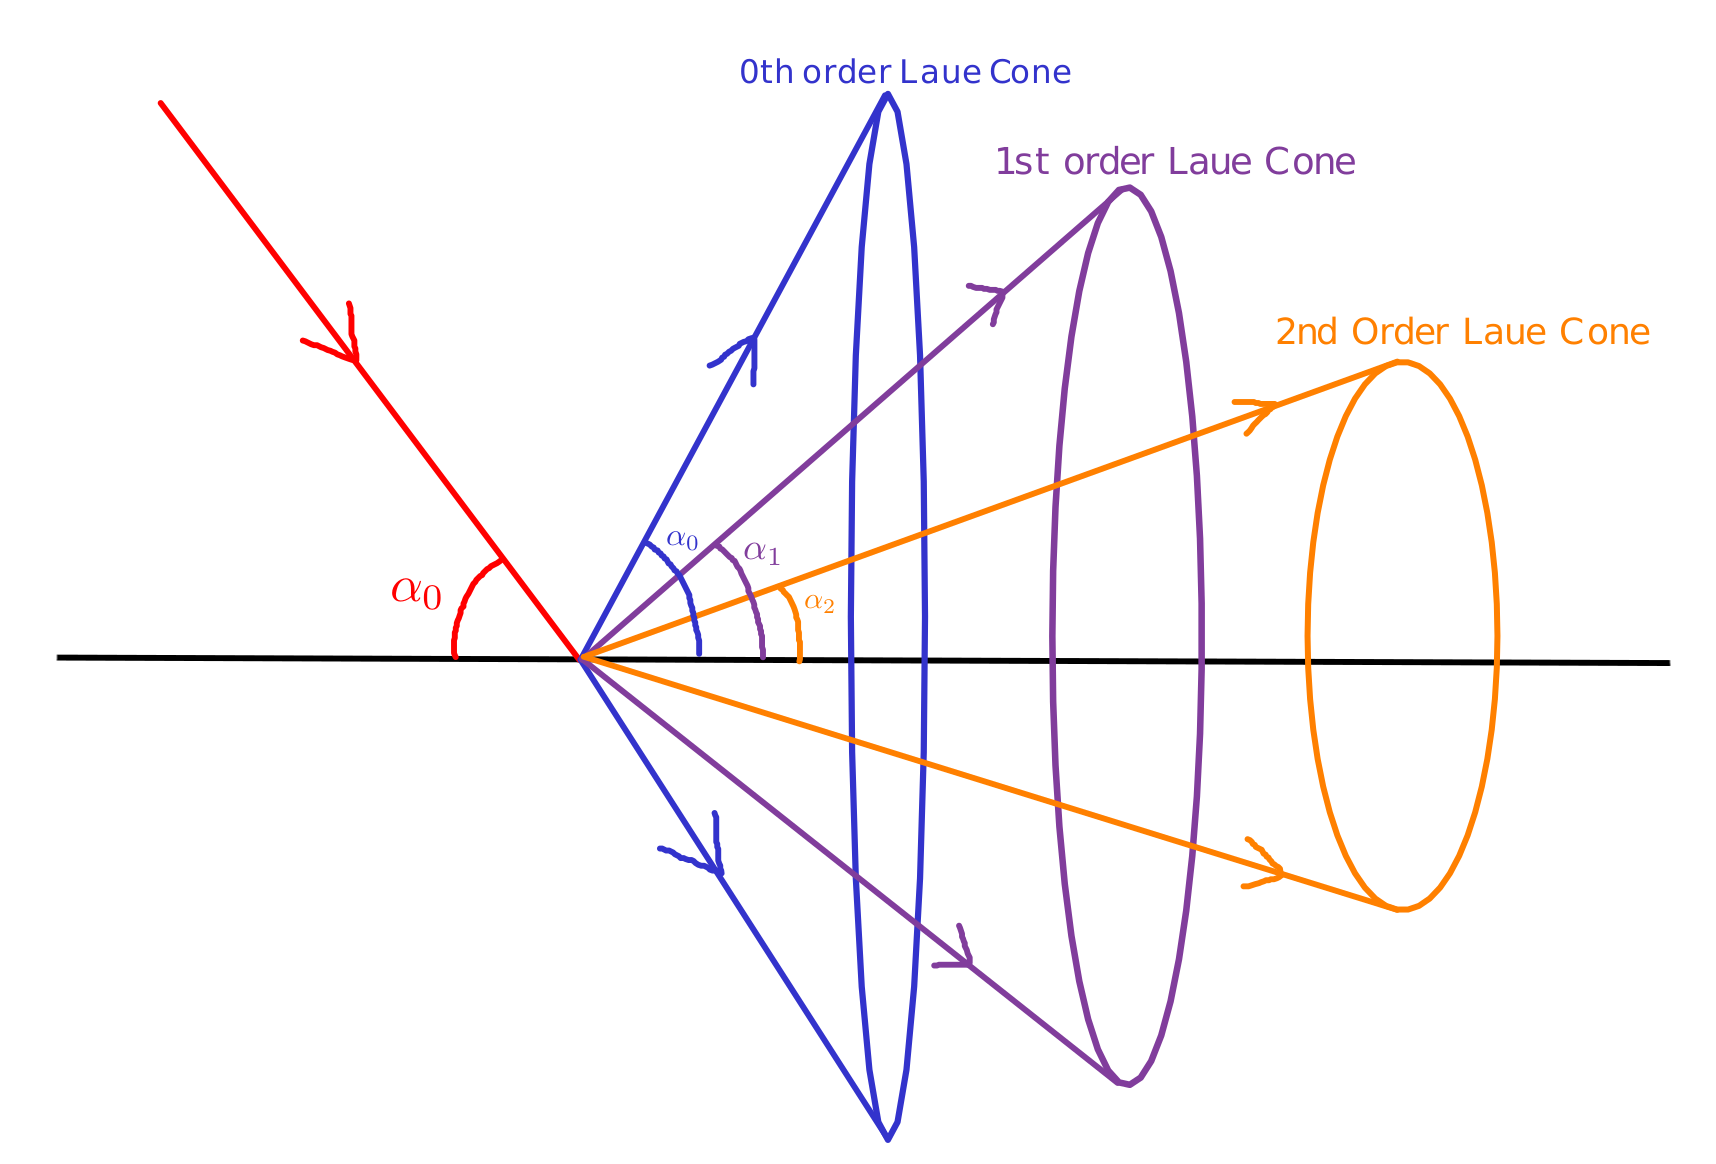
\includegraphics[scale=0.17]{laue_cones.png}
	\caption{\label{fig:laue_cones}Three Laue cones representing the direction of diffracted beam from a lattice row along the $x$-axis, with $0$ ($n_x = 0$), $\lambda$ ($n_x = 1$) and $2\lambda$ ($n_x = 2$) path differences. Similar cones also lie to the left of the 0th order cone for $n < 0.$}
	\end{figure}
	
	Proceeding similarly, we can derive two more equations for diffraction from atom rows along the $y$ and $z$ directions, thereby arriving at the second and third Laue equations:%
%		
	\begin{align}
	\boxed{b \qty( \cos \beta_n - \cos \beta_0 ) = \va{b} \cdot \qty( \vu{S} - \vu{S_0} ) = n_y \lambda,} \quad n_y \in \mathbb{Z}; \label{eq:2nd_laue_eqn} \\[1.5em]
	\boxed{c \qty( \cos \gamma_n - \cos \gamma_0 ) = \va{a} \cdot \qty( \vu{S} - \vu{S_0} ) = n_z \lambda,} \quad n_z \in \mathbb{Z}. \label{eq:3rd_laue_eqn}
	\end{align}
	
	For constructive interference to simultaneously occur from all the three atom rows in the three directions, all three Laue equations must be satisfied simultaneously. This is geometrically equivalent to three Laue cones intersecting at some points. Diffraction will only occur along those directions in which three Laue cones intersect.
	
%***********************************************************************************************

